\section{Introduction}
\begin{frame}{Introduction}
	\begin{itemize}
		\item Linear electrical systems are well researched.
		\item Analytical solutions can be found.
		\item Problems in circuit theory arise if nonlinear elements are part of the circuit.
		\item It is only natural to find a linear approximation for circuits to utilize the standard
		tool-set for circuit analysis.
		\item The approximation is only valid in a small interval; only small signals can be 
		analyzed.
	\end{itemize}
\end{frame}
\begin{frame}{Introduction}
	\begin{figure}
		\centering
		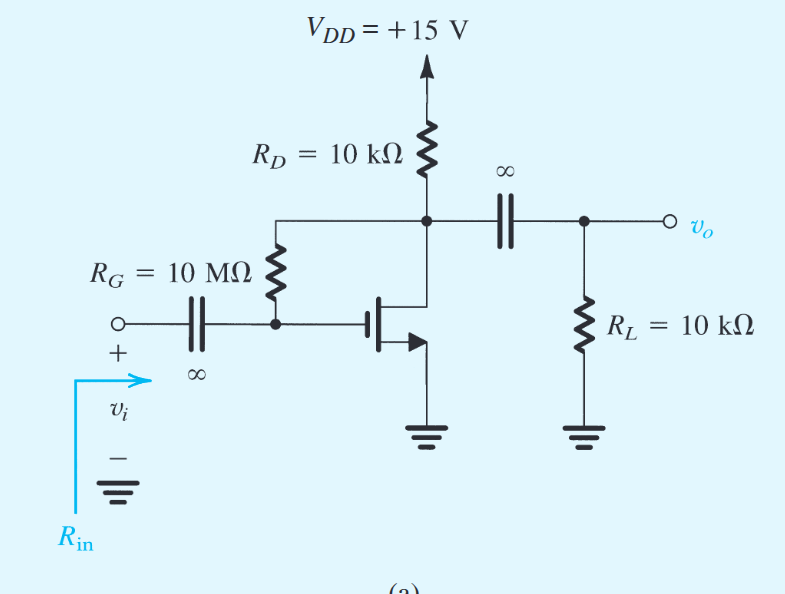
\includegraphics[width=0.7\textwidth]{../assets/example_circuit.png}
		\caption{Example circuit suitable for small signal analysis.}
		\label{fig:example_circuit}
	\end{figure}
\end{frame}